\documentclass[11pt, reqno]{amsart}

%%% Font Setup
% \usepackage{ETbb}
\usepackage{libertinus}           % text + math, type1 so pdflatex-safe
\usepackage[T1]{fontenc}

%%% Packages
\usepackage{amsmath, amssymb, amsthm}
\usepackage{xcolor}
\usepackage{bm}
\usepackage[colorlinks=true, linkcolor=blue!60!black, citecolor=blue!60!black, urlcolor=blue!60!black]{hyperref}
\usepackage{enumitem}
\usepackage{graphicx}
\usepackage{subcaption}
\usepackage{flafter}

\usepackage[framemethod=TikZ]{mdframed}
\mdfdefinestyle{lecturebox}{
  backgroundcolor=black!5,      % light gray fill
  linecolor=black!12,           % faint border; set linewidth=0pt to drop it
  linewidth=0.6pt,
  roundcorner=3pt,
  leftmargin=1em, rightmargin=1em,        % outer indent from text block
  innerleftmargin=1.4em, innerrightmargin=1.4em,
  innertopmargin=1em, innerbottommargin=1em,
}

%%% Page Geometry
\usepackage{geometry}
\geometry{margin=1.2in, top=1in, bottom=1in}

%%% Section Headings in Small Caps
\makeatletter
\def\section{\@startsection{section}{1}%
  \z@{.7\linespacing\@plus\linespacing}{.5\linespacing}%
  {\normalfont\scshape\centering}}
\makeatother

%%% Title in Small Caps
\makeatletter
\def\@settitle{\begin{center}%
  \baselineskip14\p@\relax
  \bfseries\scshape\uppercasenonmath\@title
  \@title
  \end{center}%
}
\makeatother

%%% Theorem Environments
\newtheoremstyle{notestyle}
  {6pt}{6pt}{\itshape}{}{\bfseries}{.}{.5em}
  {\thmname{#1}\thmnumber{ #2}\thmnote{ \normalfont(#3)}}

\theoremstyle{notestyle}
\newtheorem{theorem}{Theorem}[section]
\newtheorem{lemma}[theorem]{Lemma}
\newtheorem{proposition}[theorem]{Proposition}
\newtheorem{corollary}[theorem]{Corollary}

\newtheoremstyle{defstyle}
  {6pt}{6pt}{\normalfont}{}{\bfseries}{.}{.5em}
  {\thmname{#1}\thmnumber{ #2}\thmnote{ \normalfont(#3)}}

\theoremstyle{defstyle}
\newtheorem{definition}[theorem]{Definition}
\newtheorem{example}[theorem]{Example}
\newtheorem{remark}[theorem]{Remark}

\newcommand{\R}{\mathbb{R}}
\newcommand{\T}{^\top}
\newcommand{\mc}[1]{\mathcal{#1}}

%%% Additional notation
\newcommand{\E}{\mathbb{E}}
\newcommand{\V}{\mathcal{V}}
\newcommand{\Hphys}{\mathcal{H}_{\mathrm{phys}}}
\newcommand{\Cov}{\operatorname{Cov}}
\newcommand{\Tr}{\operatorname{Tr}}
\newcommand{\Id}{\mathrm{Id}}
\newcommand{\argmin}{\operatorname*{arg\,min}}
\newcommand{\norm}[1]{\left\lVert #1 \right\rVert}
\newcommand{\inner}[2]{\left\langle #1,#2 \right\rangle}
\newcommand{\MPS}{\mathcal{M}_{\chi}}
\newcommand{\Q}{\mathcal{Q}}
\newcommand{\FS}{\mathrm{FS}}
\newcommand{\Heff}{H_{\mathrm{eff}}}
\newcommand{\Neff}{N_{\mathrm{eff}}}

%%% Metadata
\title{Isosceles Perturbations of Three Correlated Cubic Features}
\author{authors}
\date{}

\begin{document}
\maketitle
\thispagestyle{empty}

\noindent\textit{%
We want to extend the three-feature calculation to a small isosceles deformation. In particular, if two teacher directions become closer to each other, how does the preferred committee representation change? We first restate the model and what the geometry means, then define the problem to work on.}

\section{Setup}

Let $N$ be the input dimension, $K$ be the number of hidden neurons,
and $P$ be the number of training examples. There are $k=3$ teacher
directions. The number of committees will be denoted by $L$ and is
not fixed in advance.

Take
\begin{equation}
 K=\frac{N^2}{\Delta},\qquad P=\chi K,
\end{equation}
with $\Delta,\chi>0$ fixed as $N\to\infty$. Our sample ratio remains
\begin{equation}
 \alpha=\frac PN=\frac{\chi N}{\Delta},
\end{equation}
so it grows with $N$. The ratio $\chi=P/K$ is fixed, and the number
of teacher directions stays equal to three.

\section{Teacher and Training Data}

Draw independent inputs $\mathbf x^\mu\sim\mathcal N(0,I_N)$.
Choose three fixed unit teacher directions
$\mathbf e_1,\mathbf e_2,\mathbf e_3\in\mathbb R^N$, and write
\begin{equation}
 z_\ell=\mathbf e_\ell^\top\mathbf x,\qquad
 G_{\ell t}=\mathbf e_\ell^\top\mathbf e_t,\qquad
 \ell,t=1,2,3.
\end{equation}
Each $z_\ell$ is a scalar measurement of the input along one direction.
It has unit variance, and
$\mathbb E_{\mathbf x}[z_\ell z_t]=G_{\ell t}$. So the Gram matrix
$G$ tells us both how the directions are arranged and how correlated
their input projections are.

Use noiseless labels
\begin{equation}
 y^\mu=f_*(\mathbf x^\mu),\qquad
 f_*(\mathbf x)=B\sum_{\ell=1}^3
 \psi_3(\mathbf e_\ell^\top\mathbf x),\qquad B>0,
\end{equation}
where
\begin{equation}
 \psi_3(z)=\frac{H_3(z)}{\sqrt6}
 =\frac{z^3-3z}{\sqrt6}.
\end{equation}
Here $H_3$ is the third probabilists' Hermite polynomial. The teacher
first projects the input along each direction, then applies a cubic
feature to that projection, then adds the three outputs with equal
strength $B$.

The projection $z$ is linear in the input, while $\psi_3(z)$ is
nonlinear. The $-3z$ term removes the linear Gaussian component of
$z^3$:
\begin{equation}
 \mathbb E_Z[Z\psi_3(Z)]=0,\qquad
 \mathbb E_Z[\psi_3(Z)^2]=1,\qquad Z\sim\mathcal N(0,1).
\end{equation}
Thus this is a pure cubic-feature problem. We have not included a
separate linear teacher feature $H_1(z)=z$.

For Gaussian inputs, the exact overlap identity is
\begin{equation}
 \mathbb E_{\mathbf x}\!\left[
 \psi_3(\mathbf e_\ell^\top\mathbf x)
 \psi_3(\mathbf e_t^\top\mathbf x)\right]=G_{\ell t}^{\,3}.
\end{equation}
So $G_{\ell t}$ is a direction overlap, and $G_{\ell t}^3$ is the
correlation between the corresponding normalized cubic features.
The student is given the dataset
$\mathcal D=\{(\mathbf x^\mu,y^\mu)\}_{\mu=1}^P$, rather than the
teacher directions themselves.

\section{Student network and equilibrium ensemble}

Use the same pure cubic student as before:
\begin{equation}
 g_i(\mathbf x)=\frac{\mathbf w_i^\top\mathbf x}{\sqrt N},
 \qquad
 f_\theta(\mathbf x)=\sum_{i=1}^K
 a_i\gamma_3\psi_3(g_i(\mathbf x)),\qquad \gamma_3>0.
\end{equation}
Here $\theta=(\mathbf a,W)$, with $W_{ij}=w_{ij}$. The hidden weight
$\mathbf w_i$ selects the direction inspected by neuron $i$, and
$a_i$ determines how strongly that neuron contributes to the output.
Both are variables of the learning problem.

The prior is uniform over hidden-weight spheres and over readouts
satisfying
\begin{equation}
 \|\mathbf w_i\|^2=N,\qquad
 |a_i|\leq\frac{A}{\sqrt K},\qquad
 \sum_{i=1}^K a_i^2=\tau^2,\qquad 0<\tau^2<A^2.
\end{equation}
Here $A,\tau,\gamma_3$ stay fixed. The norm constraint gives each
preactivation unit variance under Gaussian inputs. The readout cap
limits how much output one neuron can supply. The factor $K^{-1/2}$
has already been absorbed into our readouts $a_i$; there is no
additional normalization outside the network sum.

For fixed $\mathcal D$, define
\begin{align}
 E_{\mathcal D}(\theta)
 &=\frac12\sum_{\mu=1}^P
 [y^\mu-f_\theta(\mathbf x^\mu)]^2,\\
 p_\beta(\theta\mid\mathcal D)
 &=\frac{p_0(\theta)e^{-\beta E_{\mathcal D}(\theta)}}
 {Z_\beta(\mathcal D)},\qquad \beta=T^{-1}.
\end{align}
The posterior balances accurate predictions against prior probability.
$B$ is the teacher amplitude, while $\beta$ is inverse temperature.
The dimensionless action is
$\mathcal S_{\mathcal D}=-\log p_0+\beta E_{\mathcal D}$, up to an
additive constant.

This is an equilibrium problem. A posterior sample specifies one
complete network; it doesn't specify a training trajectory. We write
$\langle\cdot\rangle_{\mathcal D}$ for posterior averages at fixed data,
$\mathbb E_{\mathbf x}$ for averages over fresh inputs, and
$\mathbb E_{\mathcal D}$ for averages over datasets.

\section{What a committee represents}

Let
\begin{equation}
 \mathcal V=\operatorname{span}
 \{\mathbf e_1,\mathbf e_2,\mathbf e_3\}.
\end{equation}
The teacher depends only on the part of an input lying in this
subspace. A committee is a group of neurons sharing a projection into
$\mathcal V$. For neuron $i$ in committee $c$, write
\begin{equation}
 \frac{\mathbf w_i}{\sqrt N}
 =r_c\mathbf u_c+\sqrt{1-r_c^2}\,\boldsymbol\xi_i,\qquad
 \mathbf u_c\in\mathcal V,\quad
 \|\mathbf u_c\|=\|\boldsymbol\xi_i\|=1,\quad
 \boldsymbol\xi_i\perp\mathcal V.
\end{equation}
Here $\mathbf u_c$ tells us which direction the group represents,
while $0\leq r_c\leq1$ tells us how strongly its neurons concentrate on that
direction. A committee shares the first component; its neurons can
differ in their transverse components. They need not have identical
full weight vectors.

Define $\mathbf w_\ell^*=\sqrt N\,\mathbf e_\ell$. The teacher overlaps
and weight norms are
\begin{equation}
 m_{i\ell}=\frac{\mathbf w_i^\top\mathbf w_\ell^*}{N}
 =r_c\mathbf u_c^\top\mathbf e_\ell,\qquad
 q_i=\frac{\|\mathbf w_i\|^2}{N}=1.
\end{equation}
The $m_{i\ell}$ are signed alignments with individual teachers.
The norm $q_i$ is fixed here, while $r_c$ measures the part of that
norm lying in the teacher subspace. A committee can overlap with
several teachers at once; it isn't assigned to one teacher by
definition.

The useful identity is
\begin{equation}
 \mathbb E_Z\!\left[
 \psi_3(rz+\sqrt{1-r^2}Z)\right]=r^3\psi_3(z),
 \qquad Z\sim\mathcal N(0,1),
\end{equation}
with $z$ held fixed. So the part of a neuron's response that survives
averaging over transverse inputs is a cubic feature along
$\mathbf u_c$, with strength proportional to $r_c^3$.

After optimizing readout magnitudes and projection lengths as in the
original notes, write the retained cubic signal as
\begin{equation}
 f_{\mathcal C}(\mathbf x)
 =\sum_{c=1}^L b_c\psi_3(\mathbf u_c^\top\mathbf x),
 \qquad b_c\geq0.
\end{equation}
The collection $\mathcal C=\{(b_c,\mathbf u_c)\}_{c=1}^L$ describes the
committee population. Signs can be absorbed into $\mathbf u_c$
because $\psi_3$ is odd. If $n_c$ neurons contribute at readout
$A/\sqrt K$ and projection length $r_*$, then
\begin{equation}
 b_c=\frac{n_c\gamma_3Ar_*^3}{\sqrt K}.
\end{equation}
Thus $b_c$ is coherent output strength, not a neuron count. The
non-committee neurons remain as a background whose output fluctuations
are integrated out in the reduction. The function $f_{\mathcal C}$
is the retained coherent signal, not the full network output or its
posterior average.

\section{Reduced population cost}

Under the background approximation, use the same effective cost:
\begin{equation}
 F(\mathcal C;G)=\lambda\sum_c b_c+
 \frac12\mathbb E_{\mathbf x}
 [f_*(\mathbf x)-f_{\mathcal C}(\mathbf x)]^2.
 \label{eq:iso-F}
\end{equation}
The second term measures the error in the coherent signal. The first
term is the statistical cost of producing aligned neurons. Under the
spherical prior, most weights are almost orthogonal to any fixed
low-dimensional subspace, so a finite projection costs prior
probability.

For completeness, the constants carried over from that calculation are
\begin{equation}
 J(r)=-\frac12\log(1-r^2),\qquad
 r_*=\argmin_{0<r<1}\frac{J(r)}{r^3},
\end{equation}
and
\begin{equation}
 \lambda=\frac{\sqrt\Delta\,J(r_*)}
 {g_{\mathrm{eff}}\gamma_3Ar_*^3}.
\end{equation}
Here $J(r)$ is the leading alignment cost, and $g_{\mathrm{eff}}>0$
comes from integrating out the weak background. We take this
population reduction as given and hold $\lambda$ fixed while changing
the teacher geometry. $F$ is a reduced cost, distinct from both the
microscopic energy $E_{\mathcal D}$ and the action
$\mathcal S_{\mathcal D}$.

\section{The triangle and the shared direction}

Draw the three teacher vectors as arrows from the same origin.
Their tips lie on the unit sphere. Connecting those tips gives a
triangle, with side lengths
\begin{equation}
 \|\mathbf e_\ell-\mathbf e_t\|^2=2(1-G_{\ell t}).
 \label{eq:iso-distance}
\end{equation}
So larger overlap means a smaller angle between two arrows and a
shorter side between their tips. The triangle is a picture of the
teacher directions, not of training examples or hidden neurons.

\begin{figure}[htbp]
\centering
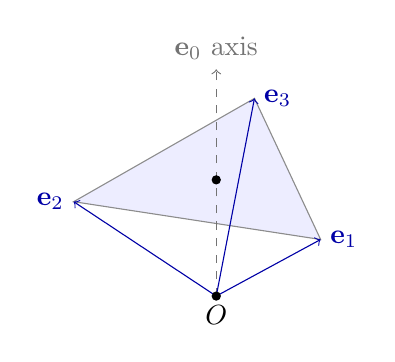
\begin{tikzpicture}[scale=2.4,
 x={(0.70cm,-0.40cm)},y={(-0.70cm,-0.40cm)},z={(0cm,1cm)}]
 \coordinate (O) at (0,0,0);
 \coordinate (E1) at (0.789,0,0.615);
 \coordinate (E2) at (-0.3945,0.6833,0.615);
 \coordinate (E3) at (-0.3945,-0.6833,0.615);
 \coordinate (C) at (0,0,0.615);
 \fill[blue!7] (E1)--(E2)--(E3)--cycle;
 \draw[black!45] (E1)--(E2)--(E3)--cycle;
 \draw[dashed,black!55,->] (O)--(0,0,1.2)
 node[above] {$\mathbf e_0$ axis};
 \draw[->,blue!65!black] (O)--(E1)
 node[right] {$\mathbf e_1$};
 \draw[->,blue!65!black] (O)--(E2)
 node[left] {$\mathbf e_2$};
 \draw[->,blue!65!black] (O)--(E3)
 node[right] {$\mathbf e_3$};
 \fill (O) circle (0.7pt) node[below] {$O$};
 \fill (C) circle (0.7pt);
\end{tikzpicture}
\caption{The equilateral case, viewed at an angle. The arrows start at
$O$; their tips form the shaded triangle. The shared axis passes
through its centroid.}
\end{figure}

The triangle lies in a two-dimensional affine plane, which generally
doesn't pass through the origin. The three vectors span the
three-dimensional linear space $\mathcal V$. A candidate committee
direction $\mathbf u$ lies on the unit sphere in $\mathcal V$; it
isn't constrained to the triangle or its plane.

In the equilateral case, every distinct pair has overlap $\omega$.
For $0<\omega<1$, define
\begin{equation}
 \mathbf e_0=\frac{\mathbf e_1+\mathbf e_2+\mathbf e_3}
 {\sqrt{3(1+2\omega)}}.
\end{equation}
This is a unit vector along the shared axis. We can write
\begin{equation}
 \mathbf e_\ell=c_0\mathbf e_0+s_0\mathbf v_\ell,\qquad
 c_0^2=\frac{1+2\omega}{3},\qquad
 s_0^2=\frac{2(1-\omega)}3,
\end{equation}
where the $\mathbf v_\ell$ are unit vectors $120^\circ$ apart in the
plane perpendicular to $\mathbf e_0$. The triangle's centroid is
$c_0\mathbf e_0$.

A candidate committee direction can similarly be written
\begin{equation}
 \mathbf u=t\mathbf e_0+\sqrt{1-t^2}\,\mathbf v,\qquad
 \|\mathbf v\|=1,\quad \mathbf v\perp\mathbf e_0.
\end{equation}
Here $t=\cos\vartheta$, where $\vartheta$ is the tilt away from the
shared axis. The direction of $\mathbf v$ specifies the azimuth of
that tilt. This angular coordinate $t$ is different from temperature
$T$, projection length $r_c$, and norm $q_i$. \color{blue}\textbf{[TODO: make a note deriving the spherical harmonics decomposition?]}\color{black}

\section{The isosceles perturbation}

Keep three teacher directions and equal feature strengths, but change
their overlaps to
\begin{equation}
 G(\omega,\delta)=
 \begin{pmatrix}
 1&\omega+2\delta&\omega-\delta\\
 \omega+2\delta&1&\omega-\delta\\
 \omega-\delta&\omega-\delta&1
 \end{pmatrix}.
 \label{eq:iso-G}
\end{equation}
The case $\delta=0$ is equilateral. For $\delta>0$, directions $1$
and $2$ are closer to each other, while direction $3$ is equally
farther from both. The average pair overlap remains $\omega$, so
we're changing the asymmetry without changing the mean overlap.

Take $|\delta|$ small enough that $G$ stays positive definite. Writing
$g_{\rm pair}=\omega+2\delta$ and $g_{\rm cross}=\omega-\delta$, this
requires
\begin{equation}
 -1<g_{\rm pair}<1,\qquad
 2g_{\rm cross}^2<1+g_{\rm pair}.
\end{equation}
We also keep both overlaps nonnegative, as in the original setup.
Strict positive definiteness keeps the teacher span three-dimensional.

The side lengths now satisfy
\begin{align}
 \|\mathbf e_1-\mathbf e_2\|^2&=2(1-\omega-2\delta),\\
 \|\mathbf e_1-\mathbf e_3\|^2
 =\|\mathbf e_2-\mathbf e_3\|^2&=2(1-\omega+\delta).
\end{align}
Thus two sides remain equal, while the side between tips $1$ and $2$
changes differently. This is what makes the triangle isosceles.

\begin{figure}[htbp]
\centering
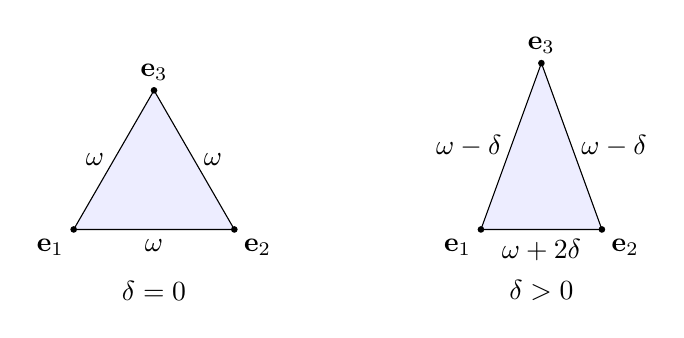
\begin{tikzpicture}[scale=1.2]
 \begin{scope}
  \coordinate (A) at (-0.85,0);
  \coordinate (B) at (0.85,0);
  \coordinate (C) at (0,1.472);
  \fill[blue!7] (A)--(B)--(C)--cycle;
  \draw (A)--node[below] {$\omega$}(B)
        --node[right] {$\omega$}(C)
        --node[left] {$\omega$}(A);
  \fill (A) circle (1pt) node[below left] {$\mathbf e_1$};
  \fill (B) circle (1pt) node[below right] {$\mathbf e_2$};
  \fill (C) circle (1pt) node[above] {$\mathbf e_3$};
  \node at (0,-0.65) {$\delta=0$};
 \end{scope}
 \begin{scope}[xshift=4.1cm]
  \coordinate (A) at (-0.64,0);
  \coordinate (B) at (0.64,0);
  \coordinate (C) at (0,1.76);
  \fill[blue!7] (A)--(B)--(C)--cycle;
  \draw (A)--node[below] {$\omega+2\delta$}(B)
        --node[right] {$\omega-\delta$}(C)
        --node[left] {$\omega-\delta$}(A);
  \fill (A) circle (1pt) node[below left] {$\mathbf e_1$};
  \fill (B) circle (1pt) node[below right] {$\mathbf e_2$};
  \fill (C) circle (1pt) node[above] {$\mathbf e_3$};
  \node at (0,-0.65) {$\delta>0$};
 \end{scope}
\end{tikzpicture}
\caption{Schematic views within the plane of the teacher tips.
Edge labels are overlaps, not lengths: a larger overlap means a
shorter side. The common arrow origin is not shown.}
\end{figure}

We can still normalize the sum of the three teacher directions after
deformation, but it no longer makes the same angle with all three.
So the equilateral common-$c_0,s_0$ decomposition doesn't carry over
unchanged. In particular, the preferred direction of a committee
serving all three features has to be found rather than assumed.

\section{Symmetry and symmetry breaking}

For equal overlaps and equal teacher amplitudes, we can permute the
three teacher directions without changing the population problem.
Geometrically, these permutations are rotations and reflections of
the triangle. There are six of them, forming the group $S_3$.
The shared axis is fixed, while vectors in the transverse plane rotate
or reflect into one another.

A symmetric problem can have symmetry-related candidate directions
that individually distinguish one teacher. If equilibrium selects
one of several symmetry-related states, this is
\emph{spontaneous symmetry breaking}: the problem stays symmetric,
but the selected state does not. An asymmetric finite posterior
sample alone doesn't establish this. Several committees may also
form a symmetric population even if each committee distinguishes a
direction.

The isosceles perturbation instead changes the problem itself.
For $\delta\ne0$, only the exchange $1\leftrightarrow2$ remains a
nontrivial symmetry, giving $S_2$. Exchanging teacher $3$ with one
member of the pair no longer preserves the overlaps. This is
\emph{explicit symmetry breaking}. It does not, by itself, tell us
how many committees will be preferred.

These symmetries apply to the population problem with Gaussian
inputs. An individual finite training set need not preserve them
exactly.

\section{Problem to work on}

Fix the teacher amplitude $B$, the student parameters, and the
effective cost $\lambda$. Start from the equilateral geometry and
introduce a small $\delta$ in~\eqref{eq:iso-G}. The question is how
the preferred representation responds when the pair $(1,2)$ becomes
closer and teacher $3$ becomes more distinct.

For a candidate direction, define
\begin{equation}
 H_\delta(\mathbf u)=
 \sum_{\ell=1}^3(\mathbf e_\ell(\delta)^\top\mathbf u)^3
 =\frac1B\mathbb E_{\mathbf x}
 [f_*(\mathbf x)\psi_3(\mathbf u^\top\mathbf x)],
 \qquad \|\mathbf u\|=1,\quad \mathbf u\in\mathcal V.
\end{equation}
This is the target--feature correlation score. Its maximizing
directions are the candidates favored at committee onset.
$H_\delta$ is distinct from the Hermite polynomial $H_3$.
For finite committee strengths, the problem is instead to minimize
$F$ in~\eqref{eq:iso-F} over the full collection $\mathcal C$.

We want to determine how the candidate directions move with $\delta$,
which remain locally stable, and which are preferred as $\omega$
is varied at a fixed small deformation. We also want to distinguish
this direction-selection question from a change in the population
at fixed $B/\lambda$, where $L$, the directions, and the strengths
are all unknown.

Here onset means that coherent committee strength first becomes
nonzero. Direction selection concerns which way an incipient committee
points. Population reorganization concerns the collection after its
strengths are finite. A crossing between competing solutions and a
loss of local stability are different events. The perturbed
directions, transition locations, and replacement populations are
left for the calculation.

% Continue here with the perturbative calculation.

\section{Small Deformation}
We hypothesize that the deformation biases representation toward the closer pair. More precisely, the three equivalent tilted branches should split into a pair associated with two teachers and a separate branch for the third. The surviving exchange symmetry forces the first two branches to remain equivalent.

Why do we maximize $H$? Let us add one committee of strength $b$ to the unaligned state. Gaussian Hermite orthogonality gives
\begin{equation}
    \mathbb E_{\mathbf x}[\psi_3(\mathbf e_\ell^\top \mathbf x)\psi_3(\mathbf u^\top \mathbf x)] = (\mathbf e_\ell^\top \mathbf u)^3,
\end{equation}
and \begin{equation}
    \mathbb E_{\mathbf x}[\psi_3(\mathbf u^\top \mathbf x)^2] = 1.
\end{equation}
Consequently, 
\begin{equation}
    F(b, \mathbf u) - F(0) = \lambda b - b \mathbb E_{\mathbf x}[f_*(\mathbf x)\psi_3(\mathbf u^\top \mathbf x)] + b^2/2 = b[\lambda - BH_\delta(\mathbf u)] + b^2/2,
\end{equation}
where $H_\delta(\mathbf u) = \sum_{\ell=1}^3(\mathbf e_\ell^\top \mathbf u)^3$. We fix $\mathbf u$ and differentiate w.r.t $b$,
\begin{equation}
    \frac{\partial F}{\partial b} = \lambda - BH_\delta(\mathbf u) + b.
\end{equation}
So 
\begin{equation}
   b_*(\mathbf u) = [BH_\delta(\mathbf u) - \lambda]_+ .
\end{equation}
And the optimized cost reduction is 
\begin{equation}
    \Delta F_*(\mathbf u) = -\frac 12 [BH_\delta (\mathbf u) - \lambda]_+^2.
\end{equation}
This identifies two things:
\begin{enumerate}
    \item onset occurs when $B\max_{\mathbf u}\, H_\delta(\mathbf u) = \lambda.$
    \item Direction selection asks which $\mathbf u$ maximizes $H_\delta$.
\end{enumerate}
A crossing between two maximizing directions can occur independently of whether the chosen $B/\lambda$ has already produced a population. Now, since the deformation is specified through the overlaps, we can use the teacher overlaps as coordinates. Define
\begin{equation}
    h_\ell = \mathbf e_\ell^\top \mathbf u.
\end{equation}
These are the committee direction's alignments with the three teachers. They differ from the microscopic neuron overlaps by the projection factor $r_c$.

Write $E = (\mathbf e_1, \mathbf e_2, \mathbf e_3)$. Since $\mathbf u$ lies in the teacher span,
\begin{equation}
    \mathbf h = E^\top \mathbf u,\quad \mathbf u = EG^{-1}\mathbf h
\end{equation}
Therefore $\|\mathbf u\|^2 = \mathbf h^\top G^{-1}\mathbf h$ and our optimization becomes
\begin{equation}
    \max_{\mathbf h} h_1^3 +h_2^3 + h_3^3 \text{ subject to } \mathbf h^\top G^{-1}\mathbf h = 1.
\end{equation}
The objective now has a fixed form, changing the teacher geometry changes the constraint ellipsoid.

Introduce a Lagrange multiplier $\Lambda$
\begin{equation}
    \mathcal L = \sum_\ell h_\ell^3 - \Lambda(\mathbf h^\top G^{-1}\mathbf h - 1).
\end{equation}
Stationarity gives us:
\begin


\end{document}
